\documentclass[12pt,a4paper,brazil,abntex2]{article}
\usepackage{lmodern}			% Usa a fonte Latin Modern			
\usepackage[T1]{fontenc}		% Selecao de codigos de fonte.
\usepackage[utf8]{inputenc}		% Codificacao do documento (conversão automática dos acentos)
\usepackage[brazil]{babel}
\usepackage{indentfirst}		% Indenta o primeiro parágrafo de cada seção.
\usepackage{graphicx}			% Inclusão de gráficos
\usepackage{microtype} 			% para melhorias de justificação
\usepackage[left=3cm,right=2cm,top=3cm,bottom=2cm]{geometry}
\usepackage{url}
\usepackage[hidelinks]{hyperref}
\usepackage{setspace}
\usepackage{cite}

%Pacotes usados na tabela inicial
\usepackage{array}
\usepackage{calc}

\newcolumntype{P}[1]{>{\centering\arraybackslash}p{#1}}
\newcolumntype{M}[1]{>{\centering\arraybackslash}m{#1}}

\usepackage[export]{adjustbox}
\usepackage{rotating}

\usepackage{multirow}
\usepackage{textcomp}
\usepackage{xcolor}
\usepackage{listings}
\lstset{
	basicstyle=\ttfamily,
	showstringspaces=false,
	breaklines=true,
  	frame=trbl,
	stringstyle=\color{black},
	identifierstyle=\color{black},
	keywordstyle=\color{red},
  	texcl=true,
  	numbers=left,
  	extendedchars=true,
  	escapeinside={(:}{:)},
  	literate=%
  		{Ç}{{\c{C}}}1
    		{á}{{\'a}}1
		{à}{{\`a}}1
		{ã}{{\~a}}1
		{é}{{\'e}}1
		{ê}{{\^e}}1
		{í}{{\'i}}1
		{ó}{{\'o}}1
		{õ}{{\~o}}1
		{ú}{{\'u}}1
		{ü}{{\"u}}1
		{ç}{{\c{c}}}1
		{É}{{\'E}}1
		{Í}{{\'I}}1
		{â}{{\^a}}1
}

\begin{document}
\singlespacing
\begin{titlepage}
\begin{center}
\begin{figure}[!htb]
\center

\includegraphics[scale=0.25]{~/Curso/Brasao/Sigla.pdf} 

\end{figure}
{\bf  UNIVERSIDADE FEDERAL DE SANTA CATARINA}\\[0.2cm] %0,2cm é a distância entre o texto dessa linha e o texto da próxima
{\bf CENTRO TECNOLÓGICO}\\[0.2cm] % o comando \\ "manda" o texto ir para próxima linha
{\bf  DEPARTAMENTO DE INFORMÁTICA E ESTATÍSTICA}\\[5.5cm]
{\bf \large IMPLEMENTAÇÃO DE COMPILADOR}\\[3.8cm] % o comando \bf deixa o texto entre chaves em negrito. O comando \huge deixa o texto enorme
{Marcos Silva Laydner}\\
{Nathan Sargon Werlich}\\
{Higor Nocetti}\\
{Sadi Júnior Domingos Jacinto}\\[0.7cm] % o comando \large deixa o texto grande
{Professor orientador: Rafael de Santiago}\\[4cm]
{Florianópolis}\\[0.2cm]
{2020}
\newpage
\thispagestyle{empty}
{Marcos Silva Laydner}\\
{Nathan Sargon Werlich}\\
{Higor Nocetti}\\
{Sadi Júnior Domingos Jacinto}\\[9cm] % o comando \large deixa o texto grande
{\bf \large IMPLEMENTAÇÃO DE COMPILADOR}\\[0.5cm]
    \begin{flushright}
    \begin{list}{}{
      \setlength{\leftmargin}{7.2cm}
      \setlength{\rightmargin}{0cm}
      \setlength{\labelwidth}{0pt}
      \setlength{\labelsep}{\leftmargin}}
      \item Trabalho prático da disciplina INE5622 – Introdução a Compiladores, consistindo na implementação de um compilador (analisador léxico e sintático), com o uso da ferramenta ANTLR4, necessário para obtenção de nota.\\[0.2 cm] 
      \setlength{\labelsep}{\leftmargin}
      \item Professor orientador: Rafael de Santiago\
      \\[8.2cm]
     \end{list}
	 \end{flushright}
{Florianópolis}\\[0.2cm]
{2020}
\end{center}
\end{titlepage} %término da "capa"
\newpage
\thispagestyle{empty}
\begin{center}
\tableofcontents
\end{center}

\section{\normalsize CONTRIBUIÇÃO DOS MEMBROS}		
	\begin{table}[h]
		\centering
		\begin{tabular}{|M{2cm}|M{5cm}|M{9cm}|}
		\hline
			{\bf{Versão}} & {\bf Participante} \	& {\bf Contribuição}\\\hline
			
 			\multirow{4}{*}[-1.65em]{\hfil 1.0} &\shortstack{Marcos Silva Laydner} & \shortstack{\\Tipos obrigatórios\\Operações obrigatórias}\\\cline{2-3}
			& Nathan Sargon Werlich & \shortstack{\\Laços \textit{for} e \textit{while}\\Estruturas de controle \textit{if-then-else} e \textit{switch-case}}\\\cline{2-3}
			& Higor Nocetti & \shortstack{\\Características adicionais da linguagem\\Códigos de teste}\\\cline{2-3}
			& Sadi Júnior Domingos Jacinto & \shortstack{\\Elaboração do Relatório\\Definição de funções}\\\hline
			\multirow{4}{*}[-1.65em]{\hfil 2.0} &\shortstack{Marcos Silva Laydner} & \shortstack{\\Operações relacionadas aos cálculos básicos\\(adição, subtração, divisão e multiplicação)\\e operação de \textit{print}}\\\cline{2-3}
			& Nathan Sargon Werlich & \shortstack{\\Não participou}\\\cline{2-3}
			& Higor Nocetti & \shortstack{\\Não participou}\\\cline{2-3}
			& Sadi Júnior Domingos Jacinto & \shortstack{\\Elaboração do Relatório, implementação das\\estruturas \textit{while}, \textit{for}, \textit{switch-case}, \textit{if-then-else},\\operações lógicas, definição e chamada de funções,\\reporte de erros semânticos, tipagem das\\funções e seus parâmetros, arquivos de teste e\\declaração e alocação de variáveis}\\\hline
		\end{tabular}
	\end{table}
	
	Importante frisar que, na primeira entrega, cada participante, além de suas respectivas contribuições, também ajudaram a testar a linguagem, além de também auxiliarem os demais colegas no desenvolvimento das outras partes do trabalho.
	
	Já na segunda entrega, apenas dois dos participantes ajudaram a testar a linguagem.
\section{\normalsize DESCRIÇÃO DA LINGUAGEM}

	A linguagem criada chama-se \textbf{sadbeep}. A mesma consiste em uma linguagem que não se utiliza de tipagem, além de apresentar a possibilidade de definições de variáveis, e um código inteiro propriamente dito, fora de funções. Além disso, a criação de variáveis não é obrigatória, visto que um código como o do exemplo abaixo é válido:

    \begin{lstlisting}
1 + 1;
"Teste de string não atribuída a nenhuma variável.";
true;
    \end{lstlisting}

    \subsection{\normalsize REQUISITOS OBRIGATÓRIOS DA LINGUAGEM}
        
        \subsubsection{\normalsize TIPOS}
            
            \begin{itemize}
                \item \textbf{INT:}\\
                    Para o tipo inteiro, foi considerado qualquer quantidade, maior ou igual à 1, de dígitos de 0 à 9, inicialmente sem limite de quantidade de dígitos.

                \item \textbf{FLOAT:}\\
                    Para o tipo de ponto flutuante, foram considerados dois grupos de dígitos, de qualquer quantidade, maior ou igual à 1 estando no intervalo de 0 à 9, concatenados por um ponto. Assim como o tipo inteiro, a princípio, não foi definido nenhuma limitação da quantidade máxima de dígitos.

                    Visando facilitar a leitura da gramática, esses dois tipos (INT e FLOAT) foram representados por um mesmo \textit{token}, chamado \textbf{NUMBER}.

                    \begin{lstlisting}
NUMBER: INT | FLOAT;
INT: [0-9]+;
FLOAT: [0-9]+.[0-9]+;
                    \end{lstlisting}
                    
        \subsubsection{\normalsize OPERADORES}
            Os operadores implementados foram baseados no código de exemplo disponibilizado no \textit{moodle}, sendo divididos em três categorias:
            \begin{enumerate}
                \item \textbf{exp:} Operações lógicas.
                    \begin{lstlisting}
exp: left=summ (op=((:\textquotesingle:)>(:\textquotesingle:) | (:\textquotesingle:)<(:\textquotesingle:) | (:\textquotesingle:)>=(:\textquotesingle:) | (:\textquotesingle:)<=(:\textquotesingle:) | (:\textquotesingle:)==(:\textquotesingle:) | (:\textquotesingle:)!=(:\textquotesingle:)) right=exp)*;
                    \end{lstlisting}

                \item \textbf{mult:} Operações de multiplicação, divisão e módulo.
                    \begin{lstlisting}
mult: left=atom (op=((:\textquotesingle:)*(:\textquotesingle:) | (:\textquotesingle:)/(:\textquotesingle:) | (:\textquotesingle:)\%(:\textquotesingle:)) right=mult)*;
                    \end{lstlisting}

                \item \textbf{summ:} Operações de adição e subtração.
                    \begin{lstlisting}
summ: left=mult (op=((:\textquotesingle:)+(:\textquotesingle:) | (:\textquotesingle:)-(:\textquotesingle:)) right=summ)*;
                    \end{lstlisting}
            \end{enumerate}

            Importante observar que a ordem de precedência dos operadores é definida pelo atributo ``\textit{left}'', indicando quais operadores tem precedência sobre quais outros. Assim, tem-se \textit{mult} com a maior precedência, seguida de \textit{summ}\footnote{graças ao uso de \textit{left=mult}}, e tendo \textit{exp} como o de menor precedência\footnote{\textit{left=summ}}.

        \subsubsection{\normalsize FUNÇÕES}
            A definição de uma função se dá com o prefixo \textit{func} seguido do nome da função, uma lista de argumentos dentro de dois parênteses, sendo possível tal lista estar vazia, e um conjunto de colchetes, dentro dos quais se encontra, obrigatóriamente, o corpo da função. A sintaxe simplicada é:

            \textbf{func nome(args) \{
                body;
            \}}

            E sua gramática é:
            \begin{itemize}
            \item[ ]
            \begin{lstlisting}
function_def : (:\textquotesingle:)func(:\textquotesingle:) name=ID (:\textquotesingle:)((:\textquotesingle:) args? (:\textquotesingle:))(:\textquotesingle:) block;
args : ID ((:\textquotesingle:),(:\textquotesingle:) ID)*;
block: (:\textquotesingle:){(:\textquotesingle:) expr* (:\textquotesingle:)}(:\textquotesingle:);            
            \end{lstlisting}
            \end{itemize}

            Sendo que a chamada de um função pode ocorrer dentro ou fora de uma função, além de permitir o uso de recursão. Para chamar uma função, basta invocar o nome da mesma, passando para ela uma lista de parâmetros, que podem ser variáveis, valores ou outras funções, A sintaxe é:

            \textbf{call\_func(args);}

            E a gramática:
			\begin{itemize}
				\item[ ]
				
    			   \begin{lstlisting}
call : name=ID (:\textquotesingle:)((:\textquotesingle:) exprs? (:\textquotesingle:))(:\textquotesingle:) (:\textquotesingle:);(:\textquotesingle:);            
	           \end{lstlisting}

			\end{itemize}
			
		\subsubsection{\normalsize \textit{IF-THEN-ELSE} e \textit{SWITCH CASE}}
        
        		\begin{itemize}
        			\item \textbf{\textit{IF-THEN-ELSE}:}\\
        				Foi seguido a estrutura clássica do \textit{if-then-else}, baseando-se na sintaxe do \textit{Java}. Inicia-se com o \textit{if}, seguido de uma condicional, que pode estar ou não contida entre parênteses, depois se encontra a abertura do par de chaves, dentro do qual se encontra o bloco que será executado caso a condicional seja verdadeira.
        				
        				Em seguida existe a possibilidade de se usar o else seguido por mais um bloco entre chaves, conforme o exemplo na seção \ref{sec3}.
        			
					\begin{lstlisting}
(:\textquotesingle:)if(:\textquotesingle:) cond=expr ((:\textquotesingle:)&&(:\textquotesingle:) cond=expr)* | ((:\textquotesingle:)||(:\textquotesingle:) cond=expr)* then-block ((:\textquotesingle:)else(:\textquotesingle:) otherwise=block)?;

block: (:\textquotesingle:){(:\textquotesingle:) expr* (:\textquotesingle:)}(:\textquotesingle:);
        				\end{lstlisting}
        			
        			\item \textbf{\textit{SWITCH}:}\\
        				Foi baseado na sintaxe do \textit{Java}, porém, sem a inclusão do bloco \textit{default} e sem a necessidade da palavra reservada \textit{break}.
        				\begin{lstlisting}
(:\textquotesingle:)switch(:\textquotesingle:) expr? (:\textquotesingle:){(:\textquotesingle:) (cases)+ (:\textquotesingle:)}(:\textquotesingle:)

cases: (:\textquotesingle:)case(:\textquotesingle:) expr (:\textquotesingle:):(:\textquotesingle:) expr (:\textquotesingle:)break;(:\textquotesingle:)?;
        				\end{lstlisting}
        		\end{itemize}
        
        \subsubsection{\normalsize \textit{FOR} e \textit{WHILE}}
        		\begin{itemize}
        			\item \textbf{\textit{FOR}:}\\
        				Foi seguida a sintaxe padrão do Java, com capacidades de atribuição, seguida da condição de parada e posterior incremento.
        				
        				\begin{lstlisting}
(:\textquotesingle:)for(:\textquotesingle:) forexpr block;

forexpr: (:\textquotesingle:)((:\textquotesingle:) variable (:\textquotesingle:)=(:\textquotesingle:) expr (:\textquotesingle:);(:\textquotesingle:) cond=expr (:\textquotesingle:);(:\textquotesingle:) variable (:\textquotesingle:)=(:\textquotesingle:) expr (:\textquotesingle:))(:\textquotesingle:);
        				\end{lstlisting}
        				
        			\item \textbf{\textit{WHILE}:}\\
        				Usada a sintaxe padrão do Java, onde existe apenas a condição de parada do laço:
        				\begin{lstlisting}
(:\textquotesingle:)while(:\textquotesingle:) cond=expr ((:\textquotesingle:)&&(:\textquotesingle:) cond=expr)* | ((:\textquotesingle:)||(:\textquotesingle:) cond=expr)* block;
        				\end{lstlisting}
        		\end{itemize}

	\subsection{\normalsize CARACTERÍSTICAS ADICIONAIS DA LINGUAGEM}
            Fora os tipos adicionais, comentados na seção de tipos, a presente linguagem apresenta, como características adicionais:
			
			\begin{itemize}
				\item Suporte à Comentários:\\
					Sejam eles de linha única ou de múltiplas linhas, seguindo a sintaxe de comentários da linguagem \textit{Java}.
					\begin{lstlisting}
//Comentário de linha única
/*Comentário longo
com mais de uma linha
*/
					\end{lstlisting}

            \begin{lstlisting}
COMMENT: (:\textquotesingle:)/*(:\textquotesingle:) .*? (:\textquotesingle:)*/(:\textquotesingle:) -> skip;
LINE_COMMENT: (:\textquotesingle:)//(:\textquotesingle:) ~[\r\n]* -> skip;]
            \end{lstlisting}
            
            		\item \&\& e $||$ Lógicos:\\
            			Foi adicionado também a capacidade de adicionar Es (\&\&) e OUs ($||$) nas condicionais das estruturas \textit{if-then-else} e \textit{while}. Sendo que o uso desses operadores pode ocorrer com o uso de duas sintaxes:
            			\begin{lstlisting}
if a > 3 && b == 0 {
...
}

if (a > 3) && (b == 0) {
...
}

while c < 1 || d == 1 {
...
}

while (c < 1) || (d == 1) {
...
}
					\end{lstlisting}
					
				\item \textbf{BOOL:}\\
                    Um dos tipos adicionais da linguagem, definido devido a utilidade do tipo \textit{booleano} em operações lógicas e condicionais utilizadas por laços como \textit{for} e \textit{while}, e por estruturas condicionais como o \textit{if-then-else}.

                    \begin{lstlisting}[language=python]
TRUE: (:\textquotesingle true\textquotesingle:);
FALSE: (:\textquotesingle false\textquotesingle:);
BOOL: TRUE | FALSE;
                    \end{lstlisting}

                \item \textbf{STRING:}\\
                    O segundo tipo adicional da linguagem, a definição de \textit{string} usada nesse trabalho comporta tanto caractéres isolados quanto textos longos. Além disso, existem dois caractéres usados para se delimitar e definir uma \textit{string}, a saber: \textquotesingle \vspace{0.1cm} e \textquotedbl.

                    \begin{lstlisting}
STRING: (:\textquotesingle:)\(:\textquotesingle\textquotesingle:)~[\r\n(:\textquotesingle:)]* (:\textquotesingle:)\(:\textquotesingle\textquotesingle:) | (:\textquotesingle:)"(:\textquotesingle:)~[\r\n(:\textquotesingle:)]*(:\textquotesingle:)"(:\textquotesingle:);
                    \end{lstlisting}
            \end{itemize}
			\end{itemize}			            
\section{\label{sec3}\normalsize EXEMPLOS DE CÓDIGOS}
	
	\begin{lstlisting}
//Tipos numéricos:
a = 2;
b = 1;
f = 0.123;
teste = 2;
	
//Boolean	
j = false;
	
//String
frase = "Teste";
	
//Função
func helloWordl() {

  //Chamar um função
  printMessage("Testando, 1,2,3");
		
  //If-then-else
  if (a > 3) {
    b = 3*(1+2);
  } else {
    a = 1.3 - 9.456;
  }
		
  //Switch
  switch teste {
    case 1:
      t = u;
    case 2:
      a = 1 + 1;
    case 3:
      l = true;
      j = false;
      break;
  }
		
  //For
  for(y = 0; y < 41; y = y + 1) {
    int = 1;
    float = 0.123;
  }
		
  //While
  while (teste < 100) {
    p = -1 + 1 * 8;
    q = (1+1)*(-8);
  }
}
	
func printMessage(message) {
  print(message);
}

helloWorld();
	\end{lstlisting}	
	\newpage
	\begin{sidewaysfigure}
	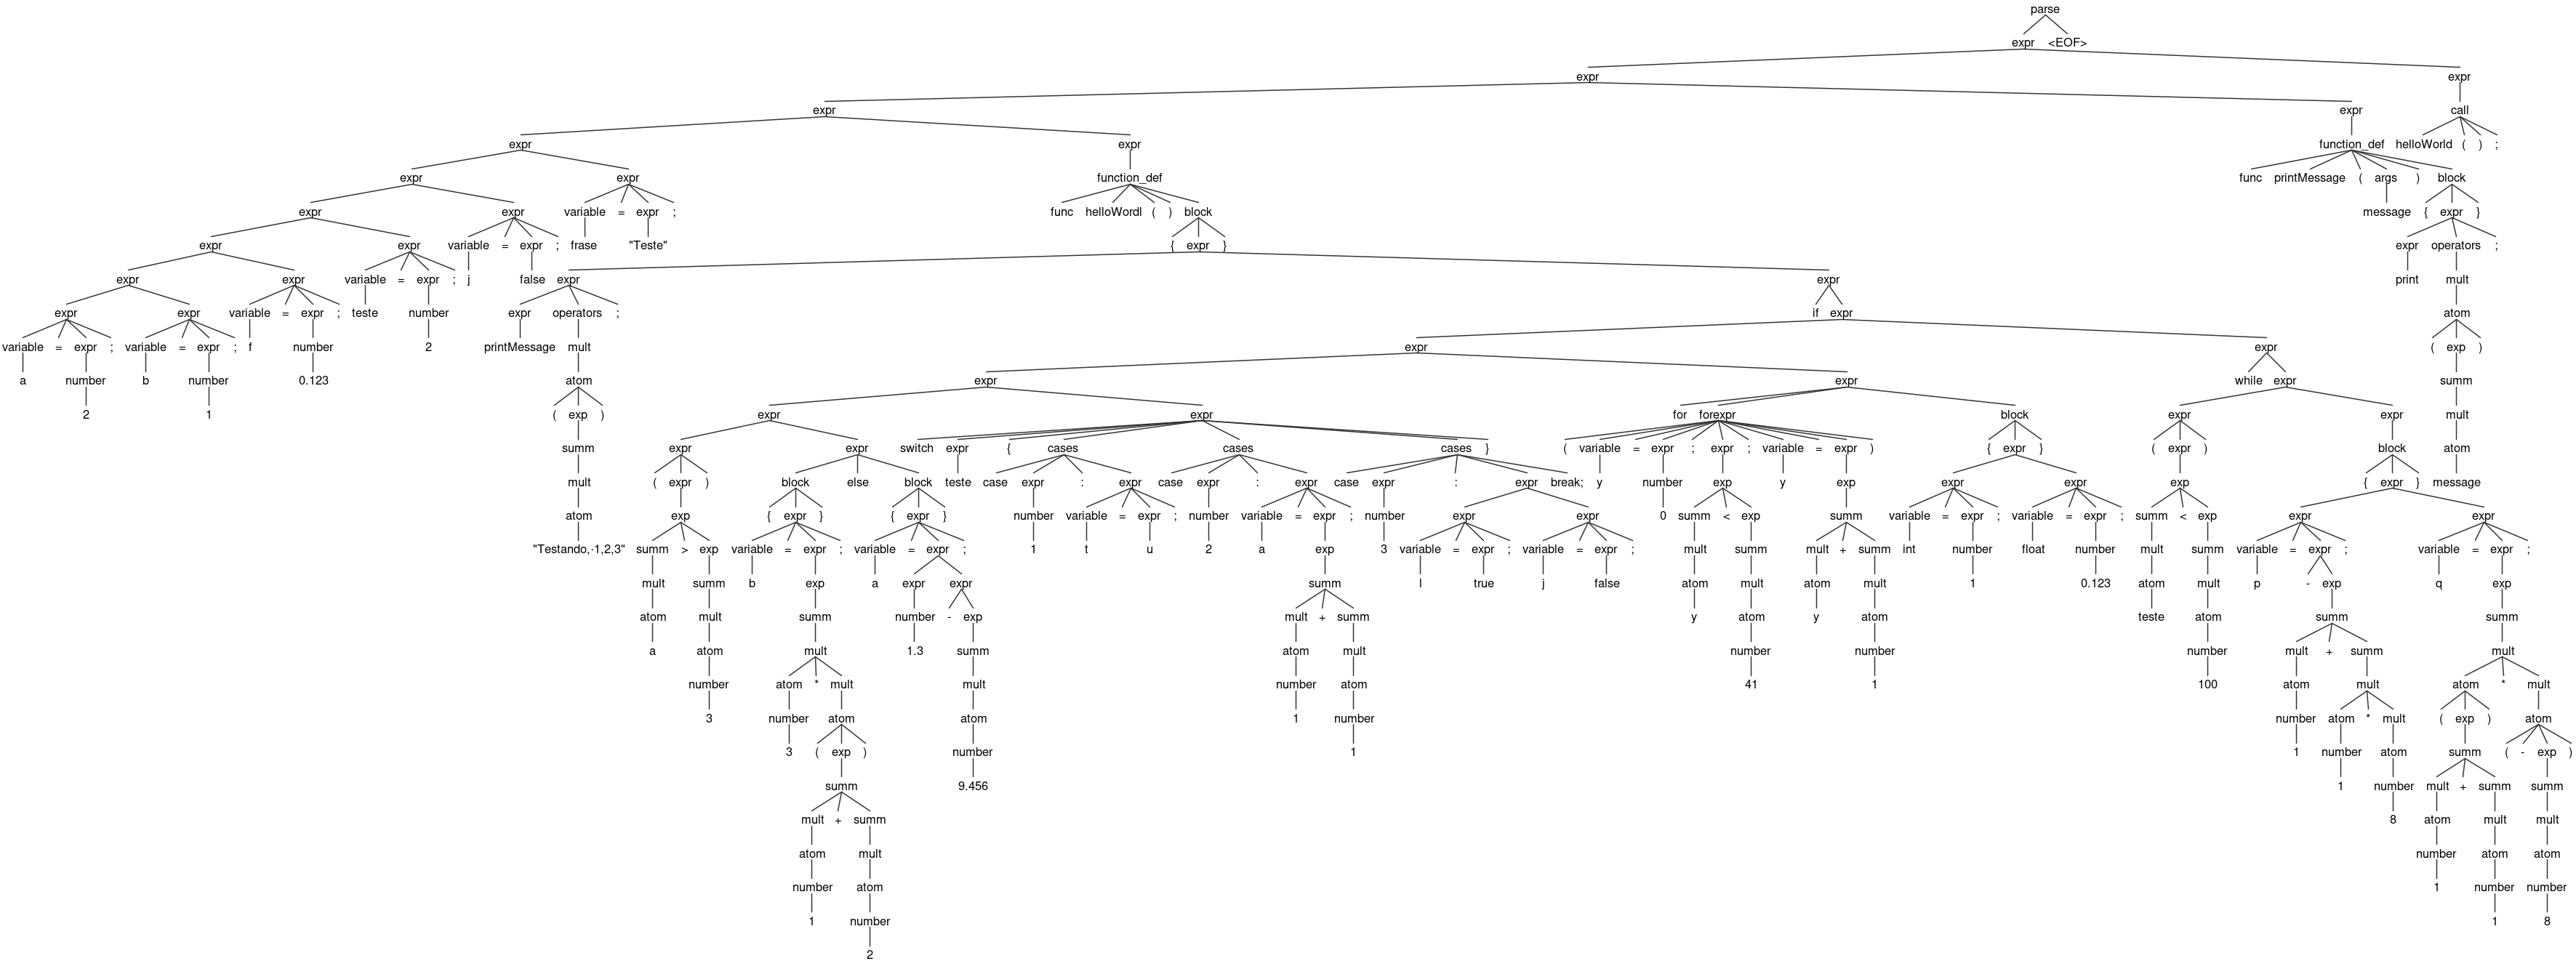
\includegraphics[width=1\textheight,height=0.8\textwidth]{01.png}
	\end{sidewaysfigure}
\section{\normalsize MUDANÇAS NA LINGUAGEM ORIGINAL}
	As seguintes mudanças ocorreram na linguagem original:
	\begin{itemize}
		\item Regra \textit{expr}:
			\begin{itemize}
				\item Foram adicionados \textit{labels} em todas as cláusulas;
				\item Foi adicionada uma nova cláusula (\textit{\textquotesingle print\textquotesingle expr \textquotesingle ;\textquotesingle});
				\item Foi removida a cláusula ID, dessa forma, a declaração de uma variável sem valor definido deixa de ser possível.
				\item Foi removida a cláusula \textit{expr operators \textquotesingle ;\textquotesingle}, uma vez que uma análise mais detalhada mostrou que tal cláusula era redundante.
				\item O símbolo \textquotesingle -\textquotesingle foi renomeado para LESS.
				\item As estruturas \textit{if} e \textit{while} foram refatoradas, uma vez que o símbolo \textbf{|} se encontrava fora dos parênteses, o que, para o ANTLR4, criava uma nova cláusula. \footnote{Exemplificando: \\antes o \textit{if} era assim:\\\textquotesingle if\textquotesingle \vspace{0.1cm} cond=expr (\textquotesingle \&\&\textquotesingle  \vspace{0.1cm} cond=expr)* | (\textquotesingle ||\textquotesingle  \vspace{0.1cm} cond=expr)$*$ then=block (\textquotesingle else\textquotesingle  \vspace{0.1cm} otherwise=block)?\\e agora ficou assim:\\ \textquotesingle if\textquotesingle \vspace{0.1cm} cond=expr (\textquotesingle \&\&\textquotesingle \vspace{0.1cm} cond=expr $|$ \textquotesingle $||$\textquotesingle \vspace{0.1cm} cond=expr)$*$ then=block (\textquotesingle else\textquotesingle \vspace{0.1cm} otherwise=block)?}
			\end{itemize}
		
		\item Regra \textit{for}:
			\begin{itemize}
				\item Basicamente a regra \textit{for} foi dividida em duas novas regras, a saber: \textit{init} e \textit{finish}.
				
				\item Para exemplificar, a antiga regra era assim:\\
				\begin{itemize}
					\item 
					
					\textquotesingle for\textquotesingle \vspace{0.1cm} forexpr block\\
				forexpr : \textquotesingle(\textquotesingle \vspace{0.1cm} variable \textquotesingle =\textquotesingle \vspace{0.1cm} expr \textquotesingle ;\textquotesingle \vspace{0.1cm} cond=expr \textquotesingle ;\textquotesingle \vspace{0.1cm} variable \textquotesingle =\textquotesingle \vspace{0.1cm} expr \textquotesingle)\textquotesingle ;
				\end{itemize}

				
				E agora a mesma é assim:
				\begin{itemize}
					\item 
					
						\textquotesingle for\textquotesingle \vspace{0.1cm} forexpr\\
						forexpr : \textquotesingle(\textquotesingle \vspace{0.1cm} init \textquotesingle ;\textquotesingle \vspace{0.1cm} cond=expr \textquotesingle ;\textquotesingle \vspace{0.1cm} finish \textquotesingle)\textquotesingle \vspace{0.1cm} block;\\
						init: variable \textquotesingle =\textquotesingle \vspace{0.1cm} expr;\\
						finish: variable \textquotesingle =\textquotesingle \vspace{0.1cm} expr;
				\end{itemize}
			\end{itemize}
		
		\item Regras \textit{args} e \textit{function\_def}:\\
			Ambas as regras foram alteradas para poderem suportar tipagem sobre o retorno da função e os parâmetros recebidos.
			
			Antes era assim:			
			\begin{itemize}
				\item
				
				function\_def : \textquotesingle func\textquotesingle \vspace{0.1cm} name=ID \textquotesingle(\textquotesingle \vspace{0.1cm} args? \textquotesingle)\textquotesingle \vspace{0.1cm} block;

				args : ID (\textquotesingle ,\textquotesingle \vspace{0.1cm} ID)*;
			\end{itemize}
			
			E agora a mesma é assim:
			\begin{itemize}
				\item 
				
				function\_def : \textquotesingle func\textquotesingle \vspace{0.1cm} name=ID \textquotesingle(\textquotesingle \vspace{0.1cm} args? \textquotesingle)\textquotesingle \textquotesingle :\textquotesingle \vspace{0.1cm} precision \vspace{0.1cm} block;

				args : ID \textquotesingle :\textquotesingle \vspace{0.1cm} precision (\textquotesingle ,\textquotesingle \vspace{0.1cm} ID \textquotesingle :\textquotesingle \vspace{0.1cm} precision)*;

				precision : \textquotesingle int\textquotesingle \vspace{0.1cm} | \textquotesingle float\textquotesingle ;
			\end{itemize}
	\end{itemize}
	

\section{\normalsize IMPLEMENTAÇÃO DO COMPILADOR}
	A implementação do compilador se baseou principalmente na linguagem de exemplo da disciplina, sendo o resto da implementação baseada em pura força-bruta\footnote{A implementação de todas as características não contempladas na linguagem de exemplo da disciplina foi por tentativa e erro.}.
	
	\subsection{\normalsize CARACTERÍSTICAS FUNCIONAIS DO COMPILADOR}
	\begin{itemize}
		\item Tipos \textit{int} e \textit{float} implementados corretamente;
		\item Possibilidade de definir e chamar funções;
		\item Estruturas \textit{if-then-else}, \textit{while}, \textit{for} e \textit{switch-case} funcionais;
		\item Operações matemáticas e lógicas funcionais, para ambos os tipos (\textit{int} e \textit{float});
		\item Toda a interface de comando (CLI) exigida.
		
	\end{itemize}
	
	\subsection{\normalsize CARACTERÍSTICAS NÃO-FUNCIONAIS}
	\begin{itemize}
		\item O reporte de erros semânticos foi implementado, e testado, apenas parcialmente, podendo haver erros ainda não detectados e/ou tratados.
		\item Fora os tipos \textit{int} e \textit{float}, nenhum outro tipo foi implementado. Além disso, somente as operações matemáticas básicas (adição, subtração, divisão e multiplicação) foram implementadas, mesmo que a definição da linguagem suporte a operação de módulo.
	\end{itemize}
	
	\subsection{\normalsize LIMITAÇÕES E ERROS DO COMPILADOR}
	\begin{itemize}
		\item Alguns erros sintáticos podem ser falsos positivos, porém, esses erros não interrompem o processo de compilação, apenas emitem uma mensagem de erro.
		\item Não é possível executar operações ou declarar variáveis fora de funções;
		\item Não é possível chamar funções dentro de funções\footnote{Exemplo: print(teste(teste2));}, nem passar para funções parâmetros que consistem em operações matemáticas ou lógicas;
		\item Obrigatoriamente deve haver uma função nomeada \textit{main};
		\item Não é possível ter duas variáveis com o mesmo nome em funções diferentes, desde que uma dessas funções seja a \textit{main};
		\item Todas as funções precisam ter \textit{return};
		\item Para uma função poder chamar a outra, a função a ser chamada precisa ser definida antes;
		\item Não é possível declarar uma variável de um tipo e depois a alterar para outro tipo;
		\item Operações de \textit{loop} usando variáveis do tipo \textit{float}, especialmente o \textit{while}, podem apresentar comportamentos estranhos, embora o resultado final apresentado não esteja totalmente errado.
	\end{itemize}
	
	\subsection{\normalsize NOTAS DO REDATOR}
	Todo o progresso de implementação do trabalho, assim como a contribuição e participação, em termos de código escrito e \textit{commits}, pode ser visualizado no seguinte repositório: \url{https://github.com/SadiJr/INE5622-Compiler}.

	Importante frisar que, a partir da postagem desse trabalho, tal repositório, antes privado, irá ter sua visibilidade alterada para público, o que pode, infelizmente, implicar em cópia por colegas desesperados.
\end{document}